\section{装好工具，先选对入口}
\label{sec:ai-desktop}

前面讲的原理可以用来选择不同厂商、不同客户端的 AI 工具。接下来，我们以 \textbf{ChatGPT 桌面版和 Codex CLI} 演示具体操作；你也可以使用已有的其他工具，按相同标准检查它能读取什么、能执行什么、怎样验证结果。先判断眼前任务需要哪种工作方式，再寻找软件中的对应入口，安装时就不会被一堆产品名绕晕。

以下软件示例的界面与命令按 \textbf{2026 年 10 月 31 日}的官方文档核对。功能会随版本、操作系统、账号方案和工作区权限变化；找不到某个入口时，先核对这些条件，再查看相应官方页面，不要照着旧教程强行寻找同一个按钮。

\subsubsection{先按任务选择工作方式，再选择客户端}

\textbf{普通聊天}适合问概念、比较思路、讨论需求，或针对一小段代码请它逐步讲解；这时你主要阅读回答，再决定下一步。需要查资料、读取实验记录、分析数据并制作报告时，可以选择支持\textbf{多步骤工具任务}的工作方式，让 AI 调用工具、读取结果后继续处理。需要进入源码工程，搜索文件、修改代码、执行命令并读取报错时，则适合具备相应工具的\textbf{代码代理（Coding Agent）}。代码代理的价值来自“查看工程—采取行动—验证结果”的循环，而不只是一次生成更长的回答。

这些工作方式没有绝对互斥的边界。同一产品可以在聊天中启用搜索、文件或代码工具，代码代理也能只讨论而不修改。判断时应查看\textbf{当前启用的工具、执行环境和权限}，不能只看产品叫“聊天”还是“代理”。在本例软件中，ChatGPT 的 \textbf{Chat} 用于对话，\textbf{Work} 用于多步骤资料与产物任务，\textbf{Codex} 提供工程开发入口；这些菜单名称并不是所有产品通用的分类。

\textbf{命令行客户端（Command Line Interface，CLI）描述的是使用入口，不是另一种模型能力。}例如 Codex CLI 是使用 Codex 的终端入口。桌面客户端适合同时看对话、文件预览、浏览器和代码差异；CLI 适合已经在终端、SSH 服务器或开发容器中工作的你。能否执行代码任务，仍取决于连接的代理、主机工具、环境、权限和资料。

\begin{center}
\begin{tabular}{p{0.23\textwidth}p{0.32\textwidth}p{0.35\textwidth}}
\toprule
通用角色与本例入口 & 适合眼前什么事 & 你应当检查什么 \\
\midrule
普通聊天，例如 ChatGPT / Chat & 解释互斥锁、比较两种接口、用小例子讲清报错 & 推理和示例是否正确，能否自己复述 \\
多步骤工具任务，例如 ChatGPT / Work & 查资料、分析实验记录、制作报告和图表 & 来源、数据口径、产物内容与版面 \\
代码代理，例如桌面版中的 Codex & 在工程中修复问题，同时查看差异与运行界面 & 修改范围、代码差异、测试和实际行为 \\
CLI 客户端，例如 Codex CLI & 在终端、SSH 或容器内使用代码代理 & 当前目录、运行主机、环境、命令和差异 \\
\bottomrule
\end{tabular}
\end{center}

\begin{example}[同一个问题，按阶段选择工作方式]
假设你的小程序偶尔卡在退出阶段。先在你使用的聊天工具中问：“用最短 C++ 例子解释条件变量为什么需要等待谓词，再让我判断一个反例。”这一步的结果应当是你能说清虚假唤醒和退出条件。在本例软件中，可以从 ChatGPT / Chat 开始。

接着，让有权访问练习副本的代码代理定位并修复，给出复现命令、预期退出方式和实际现象，要求它指出涉及的线程、锁和退出路径，并实际运行验证。在本例中可以选择桌面版的 Codex；如果工程在远程 Linux 上，也可以 SSH 到那台机器，在工程目录启动 Codex CLI。此时你检查的是工程改动，不能只收到一段“建议这样写”。切换客户端或新开聊天后，要重新确认必要结论、文件路径与复现步骤是否已提供；同一产品若能直接切换工具，也应核对当前权限和工作目录。
\end{example}

\begin{exercise}\label{ex:ai-desktop-entry}
分别为“解释引用折叠”“在板端修复 CMake 链接失败”“把三次实验的日志整理成图表”选择工作方式与合适的客户端，可以使用本例软件或已有的其他工具，并写出各自最重要的一条验收标准。说明为什么 CLI 不是另一种模型能力，为什么不能只凭产品名称判断能否操作工程。
\end{exercise}

\subsubsection{安装桌面版、CLI 与登录}

下面进入本例软件的安装与操作：\textbf{下载地址、按钮名称和 \texttt{codex} 命令只对应 ChatGPT 桌面版及 Codex CLI}。使用其他产品时，按其官方说明安装与配置，再沿用前面的任务选择和验证方法。

从\href{https://learn.chatgpt.com/docs/app}{官方桌面版指南}进入下载页，按操作系统和处理器架构选择安装包。Windows 和 macOS 用户运行官方安装程序，按照系统提示安装，然后打开 ChatGPT 并选择 \textbf{Continue to sign in}，在浏览器完成账号登录，返回应用。不要从不明网盘下载“免登录增强版”，也不要把登录令牌交给别人代为配置。

Linux 桌面版目前处于预览阶段。官方支持列表包括 Ubuntu 24.04 / 26.04 LTS、Debian 13、Fedora 43 / 44，以及完整更新的 Arch Linux，提供 x64 与 ARM64 包。\textbf{本书其他章节常用的 Ubuntu 22.04 不在这份正式支持列表内}；不方便升级时可以先使用 Codex CLI。发行版支持与限制以\href{https://learn.chatgpt.com/docs/linux/linux-app}{Linux 安装指南}为准。

\begin{example}[在受支持的 Ubuntu 上安装]
前提是 Ubuntu 24.04 或 26.04 桌面系统，且你能使用系统包管理器。先执行下面的命令确认架构：
\begin{tbash}
uname -m
\end{tbash}
若输出为 \texttt{x86\_64}，从官方 Linux 指南下载 x64 的 \texttt{.deb} 包；若为 \texttt{aarch64} 或 \texttt{arm64}，选择 ARM64 包。下面假设文件位于下载目录且使用 x64：
\begin{tbash}
cd ~/Downloads
sudo apt install ./chatgpt_amd64.deb
chatgpt
\end{tbash}
ARM64 用户把文件名换成 \texttt{chatgpt\_arm64.deb}。安装完成后应能从应用菜单启动 ChatGPT，登录后看到新建聊天入口。安装命令成功不代表模型访问已经可用，还要发送一个简单问题并确认得到回答。
\end{example}

Fedora 使用官方 \texttt{.rpm} 包及 \texttt{dnf} 安装；Arch 使用官方指南中的安装脚本。\textbf{Arch 脚本会配置签名软件仓库，并进行完整系统升级}，先按本书 Linux 维护部分做好准备，再阅读脚本、确认执行；不要把系统升级当作普通应用下载。Linux 后续通过包管理器升级应用。Linux 预览版尚不支持操作本机其他应用的 Computer Use；原生 Wayland 支持也仍在实验阶段，窗口定位和快捷键可能有差异，不需要为了学本章先改整套桌面环境。

CLI 不要求先安装桌面版。下面选用\href{https://learn.chatgpt.com/docs/codex/cli}{官方 CLI 指南}的\textbf{独立安装器}路线，它不依赖 Node.js 或 npm。已有 npm、Homebrew 或系统软件包安装的用户，先确认来源，沿原渠道升级，不要混装后再猜终端启动了哪一份。若选择 npm 路线，先按当前官方安装说明准备 Node.js / npm 与用户可写的全局安装目录；不要遇到权限错误就直接使用 \texttt{sudo npm install -g}。

\Needspace{8\baselineskip}
\begin{example}[在 Linux 或 macOS 中安装 CLI 并确认登录]
先打开终端；SSH 用户先登录\textbf{真正运行工程的主机}。检查是否已有安装：
\begin{tbash}
command -v codex
codex --version
\end{tbash}
未安装时出现找不到命令是正常现象；已有版本则先记录路径和版本，不重复安装。Linux / WSL2 用户按\href{https://learn.chatgpt.com/docs/sandboxing}{沙箱准备说明}安装 \texttt{bubblewrap}；例如 Ubuntu / Debian 上执行 \texttt{sudo apt install bubblewrap}，macOS 使用系统自带的沙箱机制。

准备好 \texttt{curl} 后，在一个新的临时目录下载安装脚本，先用编辑器查看，再以自己的普通用户执行：
\begin{tbash}
mkdir -p ~/codex-install-lab
cd ~/codex-install-lab
curl -fsSL -o codex-install.sh https://chatgpt.com/codex/install.sh
# 阅读脚本并核对来源后再运行下一行
sh codex-install.sh
\end{tbash}
目录名可换成自己尚未使用的名称。按安装器输出处理 \texttt{PATH}，然后打开新终端，确认命令位置与版本，再登录：
\begin{tbash}
command -v codex
codex --version
codex login
codex login status
\end{tbash}
浏览器登录成功后，\texttt{login status} 应报告已登录；它不能替代实际任务验证。最后进入自己的练习工程目录运行 \texttt{codex}，发送“只读说明这个项目的构建入口”，确认能获得回答且路径正确。无图形界面的 SSH 主机可在账号允许时使用 \texttt{codex login --device-auth}，在另一台设备打开终端给出的链接完成设备码登录；不要把设备码交给不可信的人。

后续升级可重新从相同官方 URL 获取并运行独立安装器，再检查 \texttt{codex --version}。其他安装渠道只执行与自己来源对应的一条：
\begin{tbash}
# npm 安装的用户使用
npm install -g @openai/codex
# Homebrew 安装的用户使用
brew upgrade --cask codex
\end{tbash}
升级后保留一次版本记录，命令发生变化时先查 \texttt{codex --help}，不要只照搬教材中的截图或旧命令。
\end{example}

Windows 可以在\textbf{原生 PowerShell}运行 CLI，也可以在 WSL2 中使用 Linux 工作流。原生方式在新的 PowerShell 窗口先用 \texttt{Get-Command codex} 检查已有安装；按官方 CLI 指南查看安装脚本后执行其安装命令：
\begin{lstlisting}[language={}]
powershell -ExecutionPolicy ByPass -c "irm https://chatgpt.com/codex/install.ps1 | iex"
\end{lstlisting}
随后在新窗口执行 \texttt{codex --version}、\texttt{codex login} 和 \texttt{codex login status}。同一命令也用于更新独立安装器版本；组织管理的设备按管理员允许的方式安装，不需要为了运行它永久放宽脚本策略。WSL2 用户在 Linux 终端中完成 Linux 安装与依赖准备，确认工程和工具链也位于所选环境；不要把 Windows 的安装成功当作 WSL 内已可用。原生 Windows 与 WSL2 使用不同的沙箱实现，详见\href{https://learn.chatgpt.com/docs/windows/windows-sandbox}{Windows 沙箱指南}。Linux 若出现 \texttt{bwrap} 或用户命名空间错误，按官方沙箱文档排查，不要通过关闭全部保护来“修好安装”。

登录时还要认清费用来源。\textbf{使用 ChatGPT 账号登录}按账号方案、额度和工作区权限使用；\textbf{使用 API Key 登录 Codex}则由 OpenAI Platform 按 API 用量计费，不会因为已经购买 ChatGPT 订阅而自动抵扣 API 消耗。API Key 方式的部分云端功能、插件连接可能不可用。本章不固定价格和额度，请查看\href{https://learn.chatgpt.com/docs/auth}{身份验证说明}及\href{https://learn.chatgpt.com/docs/pricing}{当前方案与功能表}。第一次使用先确认头像菜单中的账号和工作区，免得在个人工程里误用团队连接。

\begin{note}
API Key、登录缓存和浏览器会话都属于凭据。不要把它们贴进提示词、截图、代码仓库或求助帖；也不要把 \path{~/.codex/auth.json} 当作普通配置文件发给学长。登录出问题时提供错误信息与脱敏后的环境说明即可。
\end{note}

\begin{exercise}\label{ex:ai-desktop-install}
记录你的系统、架构、安装来源、客户端版本与登录方式；安装或检查 CLI，记录实际命令路径、\texttt{codex --version}、\texttt{codex login status} 的脱敏结果，以及今后应使用的升级渠道。若在 Ubuntu 22.04 上学习，给出一种不依赖未受支持桌面安装的路径；再说明 ChatGPT 订阅与 API Key 费用为什么要分别检查。
\end{exercise}

\section{用桌面主界面走完一次开发闭环}
\label{sec:ai-desktop-ui}

本节继续以 ChatGPT 桌面版演示。其他客户端的布局和菜单可能不同，可以按“组织任务、提供材料、执行操作、检查结果”的作用寻找对应能力，不必具有同名按钮。

\subsubsection{找到项目、聊天、输入框和检查区域}

打开应用后，先辨认四个区域。\textbf{侧边栏}用来切换项目、查找聊天和查看 Scheduled 等入口；\textbf{聊天区域}展示你的要求、代理进度、工具调用和最终结果；\textbf{输入框（Composer）}用来写任务、添加文件与图片、选择模型或输入斜杠命令；\textbf{文件、浏览器和差异区域}用来检查产物。窗口宽度和版本会改变排列，认出这些作用比背坐标更有用。

\begin{figure}[H]
    \centering
    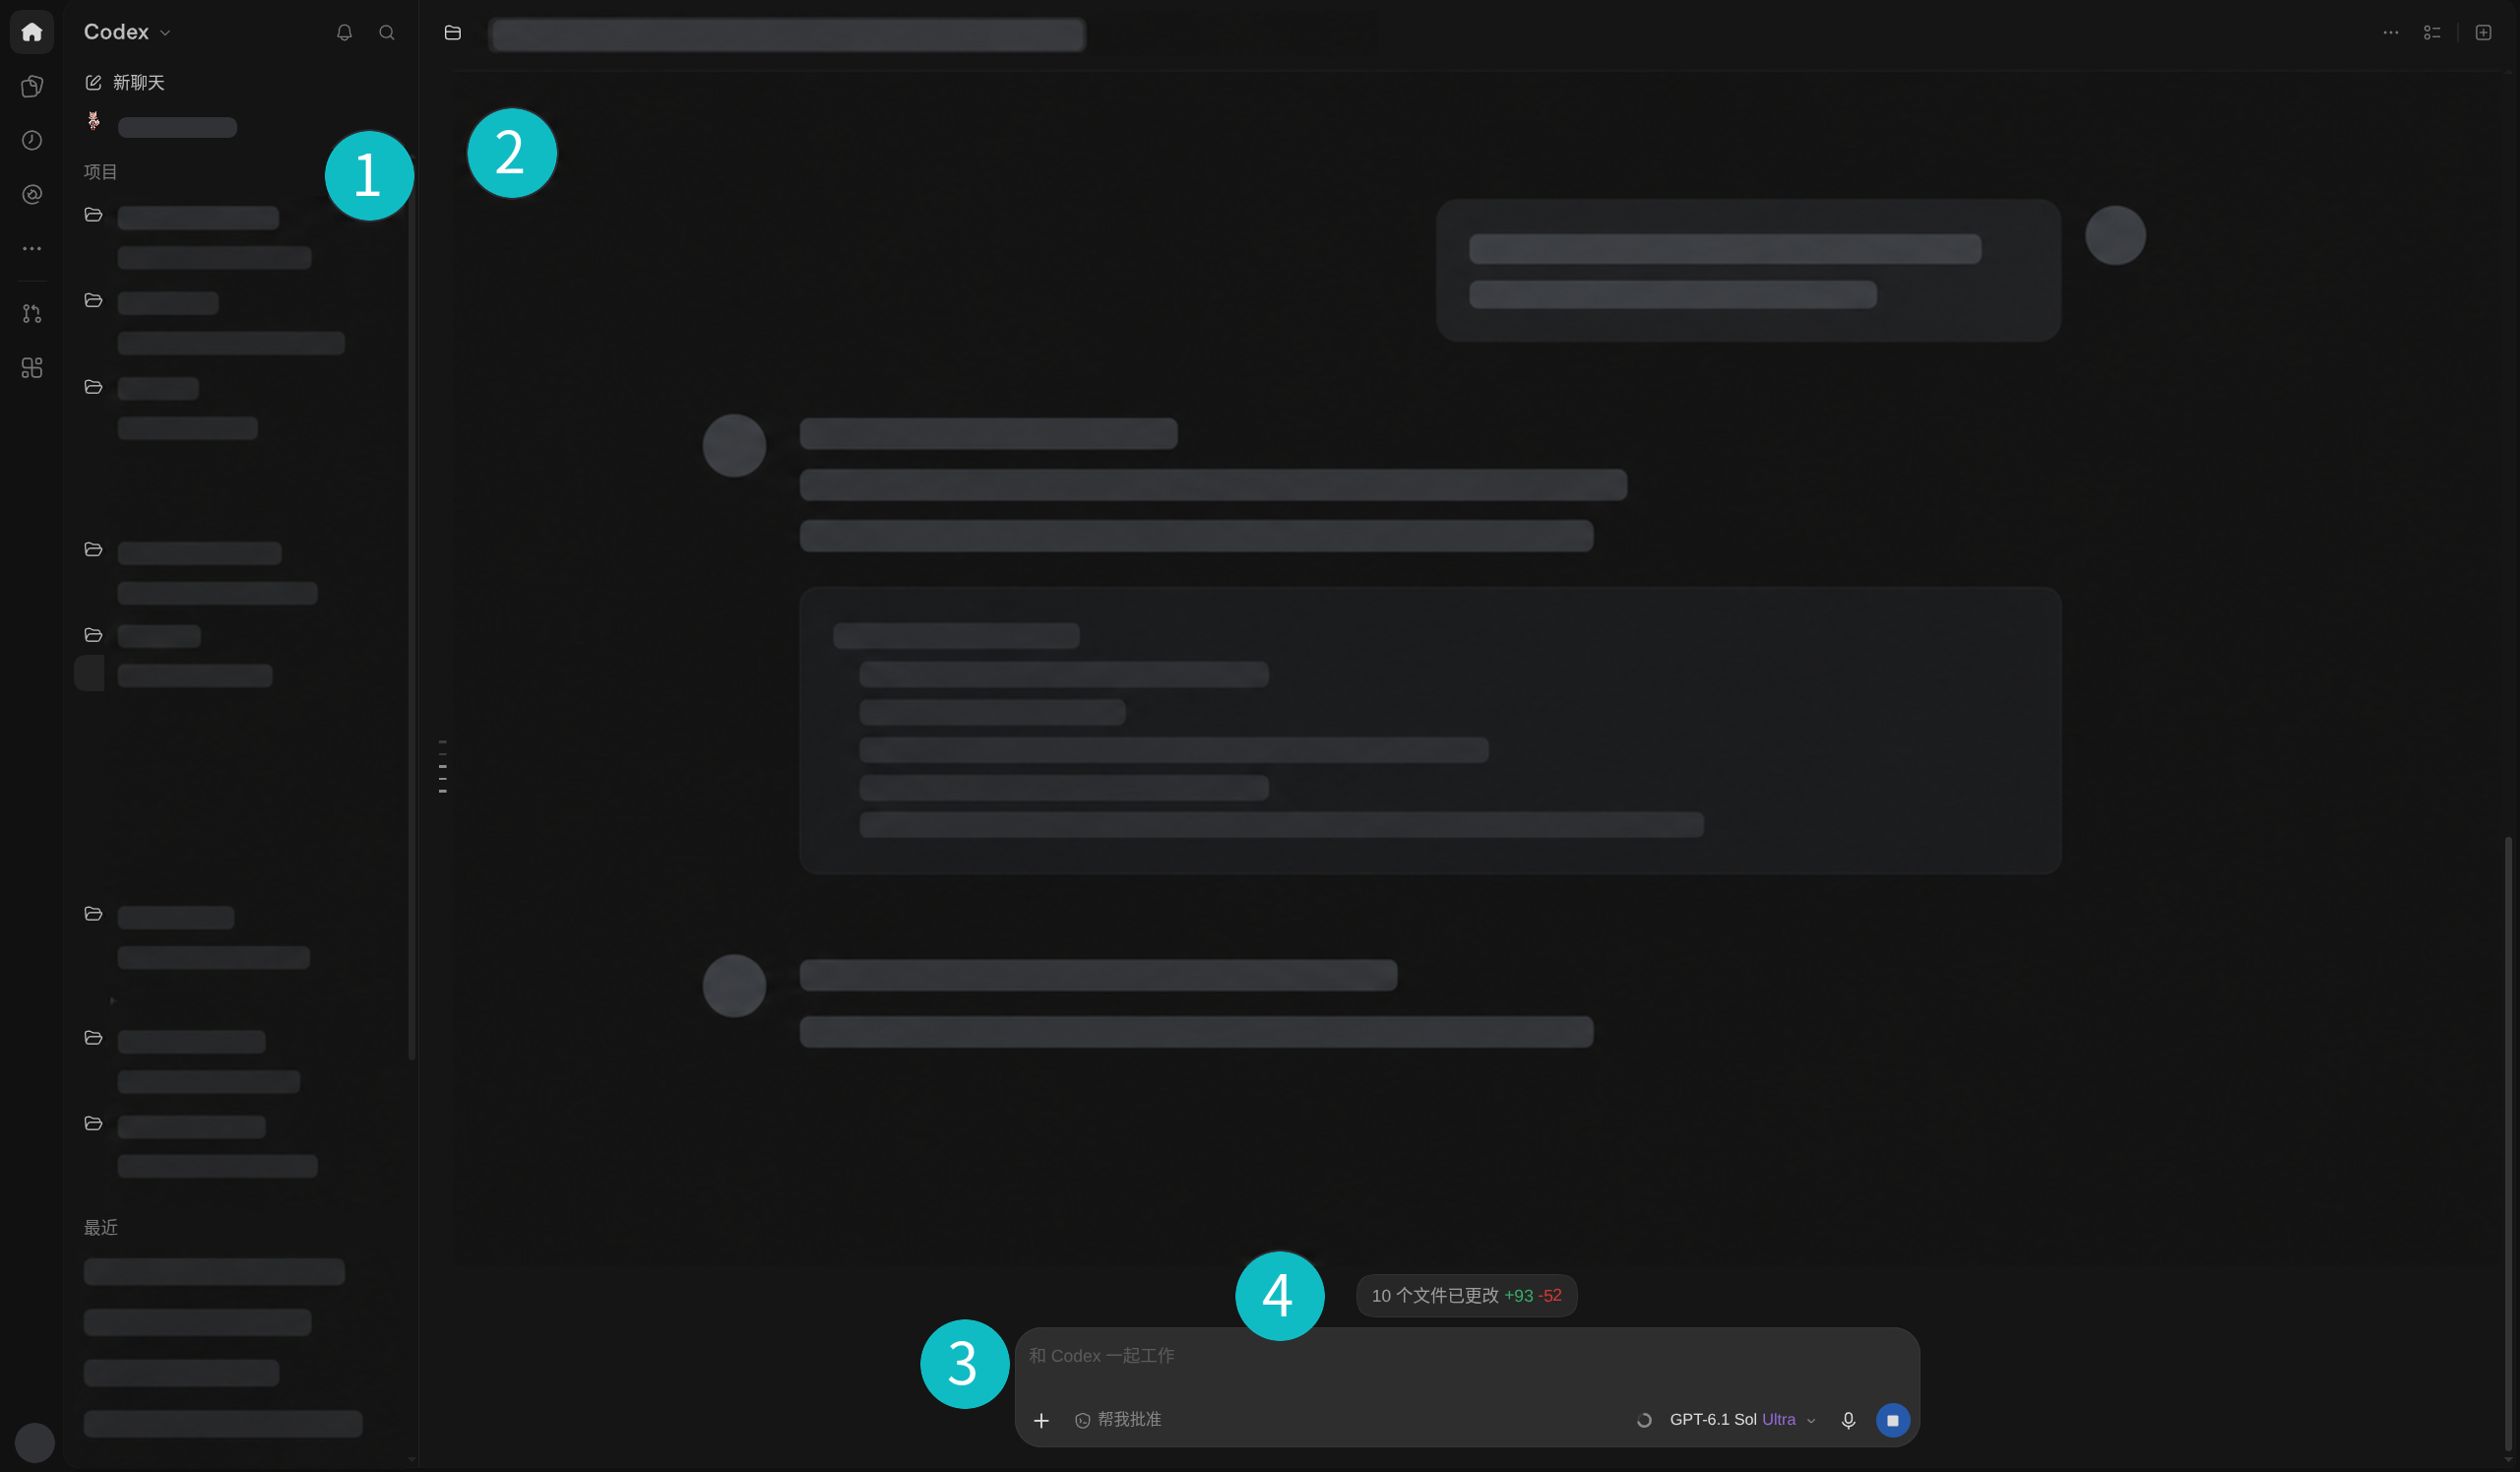
\includegraphics[width=0.98\textwidth]{images/ai/desktop-overview_revised.png}
    \caption{本机 Linux 桌面版的 Codex 入口，2026-10-31 实际截图。1：项目与聊天栏；2：对话区域；3：输入区；4：文件改动入口。项目名、标题、正文和头像以骨架占位脱敏，数字为教材标注。}
    \label{fig:ai-desktop-overview}
\end{figure}
先在图~\ref{fig:ai-desktop-overview}~中找到 1--4，再对照自己的软件。图里的圆角灰条是脱敏用的骨架占位，并非软件正在加载；实际使用时会显示项目名称和对话内容。选择项目以后，输入区上方的改动入口可以带你进入差异面板。

新建聊天时，在产品下拉菜单选择 \textbf{ChatGPT} 或 \textbf{Codex}。选择 ChatGPT 后，输入框上方可切换 \textbf{Chat / Work}；做工程任务则选择 Codex。模型菜单用于选模型及可用的思考等级；\texttt{/status} 用于确认当前聊天的状态。想先讨论再实施时使用计划模式；要持续推进较长任务时再考虑目标，见第~\ref{sec:ai-workflow}~节。

\begin{figure}[H]
    \centering
    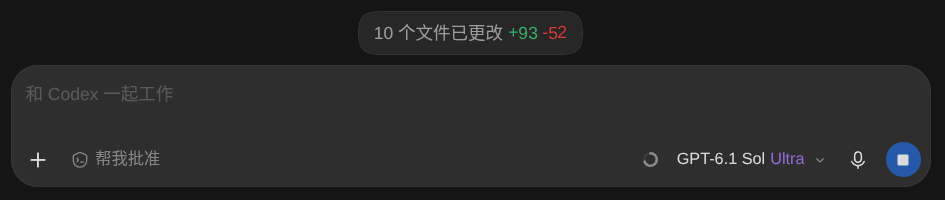
\includegraphics[width=0.98\textwidth]{images/ai/composer-controls_revised.png}
    \caption{输入区的真实局部截图：左侧为添加上下文与权限入口，右侧为模型/模式、语音及停止控件。截图时任务正在运行，蓝色方块用于停止；图中的型号和模式仅代表本机选择。}
    \label{fig:ai-composer-controls}
\end{figure}
图~\ref{fig:ai-composer-controls}~把输入区放大了。先看当前选了什么、任务是否正在执行，再发送要求；具体型号和模式名称随产品与版本变化，选型方法仍回到第~\ref{sec:ai-model-choice}~节。

\textbf{项目（Project）负责组织相关聊天和资料，聊天（Chat）负责一个具体结果。}例如把视觉工程放在一个项目中，再分别建“修复串口退出”“测量图像拷贝耗时”“审查时间戳接口”三个聊天。给聊天改一个能识别结果的名字，正在处理的可以置顶，完成的归档；归档后可从 Settings 的 Archived chats 找回。置顶只改变显示位置，不会让模型额外读到资料。

要修改本地代码，需要创建或编辑\textbf{本地项目}，附加正确的工程文件夹。普通 ChatGPT 项目中的上传资料与本地磁盘目录不是同一件事。一个本地项目可附加多个文件夹，但主文件夹决定默认工作目录、Git 操作以及自动发现项目规则的位置；其他文件夹虽然可被读写，却不会因此自动加载其中的项目指令。多工程协作时先确认主目录，别把“打开了文件夹”误当成“已经读懂全部代码”。这些行为可查\href{https://learn.chatgpt.com/docs/projects}{项目与聊天指南}。

\Needspace{7\baselineskip}
\begin{example}[先证明代理看到了正确工程]
复制本卷一个随书示例到自己的练习目录，在桌面版创建本地项目并附加该目录，选择 Codex。先发送：“只读检查这个项目：告诉我当前工作目录、Git 分支、构建入口和一个关键源文件的路径，暂不修改。”把返回路径与自己的文件管理器对照，查看它确实读取过哪些文件。

随后通过附件入口添加一份脱敏报错，或在输入框中引用具体文件；截图适合补充界面现象，编译错误最好同时提供可复制的原文。让它列出复现命令，与你实际执行的命令一致后再开始修复。完成标志是目录、文件、环境与复现步骤都已对应，不能只看一句“我看过项目了”。
\end{example}

\begin{exercise}\label{ex:ai-desktop-project}
创建一个练习项目，为两个不同结果分别建立并命名聊天；在其中一个聊天附加文件，请代理报告实际读取的路径。解释为什么“聊天已同步到另一台机器”不能证明那台机器也拥有你的本地源码。
\end{exercise}

\subsubsection{边工作边检查：终端、差异、审查与提交}

代理执行时，会在聊天中显示正在搜索、修改或运行什么。需要纠正方向就给出新的具体约束；需要停止则使用停止控件，随后检查已经产生的文件与进程。停止生成不等于撤销此前的改动。发送中的补充消息是立即引导当前工作还是排到下一轮，可在 Settings 的 Follow-up behavior 中设置，发送前留意界面提示。

在项目中通过 \textbf{New tab → Terminal} 打开集成终端。终端位于当前项目或 worktree，可用来独立运行构建命令、查看失败输出以及检查 \texttt{git status}。它不是另一个隔离副本；你在终端改文件，代理也会看到。把经常使用的构建、测试和启动命令配置为本地环境的 \textbf{Actions} 后，可以从顶栏快速执行；\textbf{Setup script} 则是在创建 worktree 时准备依赖的步骤，不应把启动开发服务器这种长期进程混进去。安装脚本、依赖和 Actions 本身也要检查，详见\href{https://learn.chatgpt.com/docs/environments/local-environment}{本地环境指南}。

代码改完以后，打开\textbf{差异面板（Diff / Review pane）}逐文件阅读。这里展示的是 Git 检出目录的状态，可能同时包含你自己、代理或其他工具的修改。按需切换 \textbf{Unstaged}、\textbf{Staged}、\textbf{Branch}、\textbf{Last turn} 等范围，别把“当前所有未提交改动”都算成代理刚刚写的。你可以对具体行留下评论，再在聊天中明确要求处理；也可以按块或按文件暂存、取消暂存、撤销修改。

\begin{figure}[H]
    \centering
    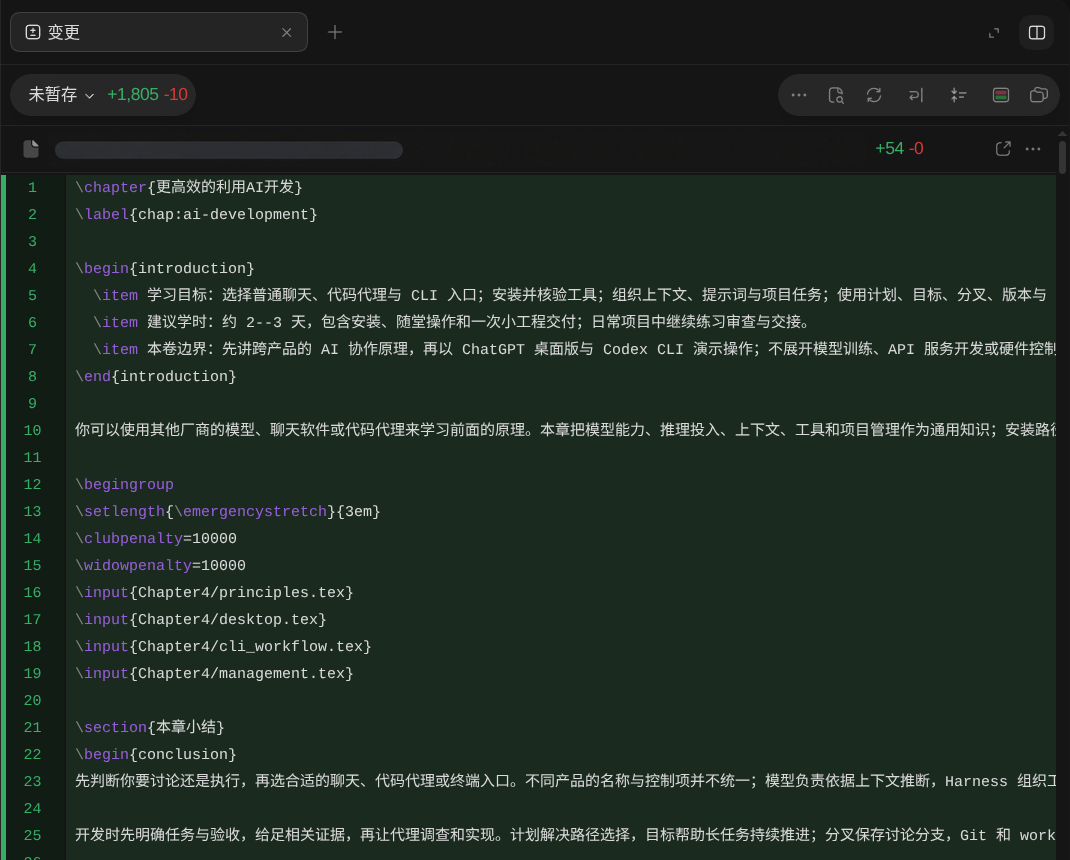
\includegraphics[width=0.92\textwidth]{images/ai/review-pane_revised.png}
    \caption{本机差异面板的真实局部截图。顶部“未暂存”表示查看范围，文件头与行号帮助定位，绿色部分是新增内容。文件路径以骨架占位脱敏，代码和计数保持原样；界面计数不是测试结果。}
    \label{fig:ai-review-pane}
\end{figure}
图~\ref{fig:ai-review-pane}~中整段为绿色，是因为这里正在查看新加入的教材文件。普通修改还可能出现删除行与修改块；先确认查看范围，再沿行号阅读，不能看到绿色就默认应该保留。

\texttt{/review} 会对选定范围进行代码审查并报告可疑问题。让它优先解释“什么输入触发、实际会怎样、预期应怎样、证据在哪”，再去核对代码与测试。审查没有发现问题，只表示这一轮没找到，不能替代构建、测试和实机验收。准备保留的改动确认后，再提交（Commit）；推送（Push）、创建 PR 和合并会影响远端，操作前要检查目标分支、内容与团队流程。\href{https://learn.chatgpt.com/docs/code-review}{审查指南}同时说明了本地审查与 PR 审查的区别。

\begin{note}
\textbf{Revert 会丢弃所选未提交改动。}先读差异，确认没有自己的工作被混在里面；需要保留的方案先提交到分支。对话分叉、对话回退与文件回退的区别见第~\ref{sec:ai-workflow}~节，不能把聊天当作 Git 备份。
\end{note}

\Needspace{8\baselineskip}
\begin{example}[检查一个“看上去已经修好”的补丁]
让代理在练习副本中完成一个小改动后，先打开差异面板，确认只涉及任务所需文件；在关键行留下一条评论：“请解释空输入为什么走这条分支，并给出能覆盖它的命令。”发送后，核对解释与实际代码。

再在集成终端亲自执行项目 README 中的构建和相关测试命令。若失败，将完整命令、退出码与关键报错给代理，继续修复；通过后执行 \texttt{/review} 并选择未提交修改。最后检查差异、测试结果和已知限制，再暂存与提交。完成标志是一份你能解释且经过验证的补丁，而不是“AI 说它测过”。
\end{example}

\begin{exercise}\label{ex:ai-desktop-review}
在练习副本中检查一份补丁，找到一处关键逻辑并留下精确到行的反馈。记录一次实际验证的命令和结果，区分差异检查、AI 审查、运行测试分别能发现哪类问题。
\end{exercise}

\subsubsection{按任务增加文件、浏览器、远程环境和定时工作}

主界面的其他功能也应当围绕“提供证据、采取行动、检查结果”使用，而不是开得越多越厉害。

\begin{center}
\begin{tabular}{p{0.20\textwidth}p{0.36\textwidth}p{0.34\textwidth}}
\toprule
功能 & 什么时候用 & 使用时要说清楚 \\
\midrule
文件与图片输入 & 分析日志、图表或截图中的现象 & 来源、时间、相关文件和要检查的位置 \\
联网搜索 & 查新版 API、安装支持与近期变更 & 优先官方来源，返回链接及适用版本 \\
产物预览 & 查看生成的文档、表格、图片 & 检查内容、单位、样式，导出后再核对 \\
内置浏览器 & 验证网页界面、复现操作 & URL、页面状态、操作与预期结果 \\
Computer Use & 任务只能通过应用界面完成 & 允许的应用、动作与确认边界 \\
Local / Cloud / 远程连接 & 选择实际执行工程的环境 & 主机、目录、依赖、网络和可用设备 \\
Scheduled & 稳定、可重复的检查或报告 & 频率、范围、通知条件和停止条件 \\
Memories & 在可用时复用过往偏好与背景 & 重新核实会变化的事实，项目决定仍入库 \\
\bottomrule
\end{tabular}
\end{center}

浏览器里“看着没问题”和浏览器真的执行过操作是两件事。桌面版的 \textbf{New tab} 可打开内置浏览器；让代理使用 \texttt{@Browser} 查看明确的本地网址，在页面上通过 \textbf{Annotate} 给具体元素加反馈，然后回到聊天要求修复并再次检查。内置浏览器的登录配置与日常浏览器分开；需要使用已有 Chrome / Edge 等标签页时，按\href{https://learn.chatgpt.com/docs/chrome-extension}{官方浏览器扩展指南}连接。\textbf{Codex CLI 没有桌面版内置浏览器}；CLI 若需要网页自动化，要另行配置支持的工具，或切回桌面版。网页搜索也不等于操作浏览器。

\textbf{本地、云端与远程}首先区别在“代码和命令实际在哪里执行”。本地任务使用你选择的文件夹与本机依赖；云端任务需要准备可访问的仓库、依赖和环境，不能默认能访问本机相机、串口或未上传文件；远程连接使用另一台已连接主机的文件和工具。同步聊天记录不等于同步源码或硬件。每次切换后，先确认主机与目录，再跑最小环境检查。平台和工作区也会影响 Computer Use、浏览器及云端功能的可用性，按实际权限使用。

\begin{example}[手动检查稳定以后，再安排定时工作]
在能访问练习仓库的桌面聊天中，先手动发送：“只读检查最近一天的提交，按功能概括变化；若构建记录显示失败，列出提交与证据链接。没有新变化则无需通知。”确认它取到正确仓库和记录后，再要求：“每个工作日 20:00（Asia/Shanghai）执行，结果回到这个聊天；连续一周后停止，不自动提交或推送。”

在 \textbf{Scheduled} 中检查保存的提示词、时间、环境、状态和下一次运行，先手动试跑并检查最初几次结果。涉及本地文件时，需要机器开机、应用运行、项目目录仍可用；有修改的周期任务宜使用独立 worktree。任务不再需要时暂停或删除。CLI 没有 Scheduled 管理界面，不能把 \texttt{codex exec} 当作已自动安排好的周期任务。
\end{example}

\begin{exercise}\label{ex:ai-desktop-tools}
为“检查本地调参网页的按钮错位”写出包含网址、窗口大小、操作和结果判断的任务；再为“每晚汇总构建失败”写出频率、证据、通知条件和停止条件。说明两项任务各自需要什么环境，哪些条件不能由聊天同步自动补齐。
\end{exercise}

\begin{conclusion}
先用项目和目录确定工作范围，用附件、搜索和连接补充证据，再通过差异、终端和预览检查结果。模型选择改变思考能力与成本；工具和环境决定它能看到什么、能执行什么。后者没有准备好，继续提高思考等级也不会凭空得到一台相机。浏览器、定时工作和环境说明分别见\href{https://learn.chatgpt.com/docs/browser}{浏览器指南}、\href{https://learn.chatgpt.com/docs/automations}{定时任务指南}与\href{https://learn.chatgpt.com/docs/reference/settings}{设置参考}。
\end{conclusion}

\section{用插件与 MCP 接入开发资料和工具}
\label{sec:ai-plugins}

\subsubsection{先分清插件、连接与 Skill}

遇到资料在 GitHub、任务在 issue 系统、设计记录在团队文档里的情况，不必反复复制整屏内容。\textbf{插件（Plugin）}把可安装的能力打包，可能包含 Skills、MCP 工具或其他组件；\textbf{连接器（Connector）}负责接入外部服务及其账号；\textbf{模型上下文协议（Model Context Protocol，MCP）}是代理与外部工具、资料提供方交互的标准。\textbf{Skill}则主要规定某类任务该按什么步骤做。一个插件可以既带“怎样审查”的 Skill，也带“获取 PR”的工具，但安装说明书不会自动获得 GitHub 权限。

桌面版从 \textbf{Plugins} 打开目录，搜索插件、阅读发布者与能力说明，选择安装；需要账号的连接按提示认证。随后\textbf{开始新聊天}，从输入框的 \texttt{@} 菜单选中插件或其 Skill，写清目标。Codex CLI 中用 \texttt{/plugins} 浏览配置允许的市场，安装后同样开始新会话；不要假定所有桌面插件都能在 CLI 运行。可通过 \texttt{/mcp} 核对实际可调用的服务器和工具。若工具缺失，依次检查是否安装、是否启用、是否已连接账号、当前账号有无目标资料权限，再检查平台支持。详见\href{https://learn.chatgpt.com/docs/plugins}{插件安装与权限指南}。

\begin{center}
\begin{tabular}{p{0.22\textwidth}p{0.34\textwidth}p{0.34\textwidth}}
\toprule
常见能力 & 开发时怎么用 & 一个明确的请求 \\
\midrule
GitHub / Code Review & 读取 issue、PR、差异、检查结果，辅助审查 & 对照 issue 验收点检查指定 PR，给出证据，先保留评论草稿 \\
OpenAI Docs / 文档 MCP & 查询官方接口与安装文档 & 查当前接口的参数要求，实际打开文档并附链接 \\
Browser / 浏览器工具 & 复现网页行为并检查渲染结果 & 在指定页面完成操作，比较修复前后的状态 \\
Linear 等任务系统 & 读取需求、依赖和状态，整理待办 & 汇总分配给我的阻塞任务及关联 PR，不修改状态 \\
Google Drive 等文档连接 & 读取设计资料与实验记录，形成交付文档 & 从指定记录提炼接口约定，标明来源与冲突 \\
Codex Security & 在授权仓库中检查潜在安全问题 & 扫描练习仓库，复核可疑输入路径与证据 \\
\bottomrule
\end{tabular}
\end{center}

这张表按能力选用，不要求全装；具体名称和可用性以当前目录为准。普通的构建、Git 本地操作和文件搜索通常已有工具，先把它们用好。只有确实需要外部资料或服务时才增加连接，减少无关工具和账号带来的干扰。

\begin{example}[用 GitHub 资料审查一次修复]
前提是你有一个可访问的练习仓库和 PR。安装或启用相应 GitHub / Code Review 能力，连接具有该仓库访问权限的账号；开始新聊天，选择该插件，提供 PR 链接，并要求：“读取 PR 和对应 issue，只检查空输入处理是否满足验收。给出涉及文件、触发条件和测试证据；评论先写成草稿。”

桌面版 \textbf{Code Review} 中可打开 PR 的 \textbf{Summary} 查看描述与检查，切到 \textbf{Changes} 查看差异。把回答引用的行和测试与当前版本对照。能读到 PR 说明和差异，才算连接可用；只有一句概括不够。确认意见后再决定是否发布评论或提交审查。\textbf{在 PR 页面发布评论会写入外部系统}；检查对象、文字和权限后再执行，不能把“帮我看看”自动升级成“替我批准并合并”。
\end{example}

\subsubsection{亲手连接一个只读文档 MCP}

MCP 服务器可以是本机命令启动的 \textbf{STDIO} 进程，也可以是通过 URL 访问的 \textbf{Streamable HTTP} 服务。前者需要本机安装运行时与命令，后者需要网络，部分还需要 OAuth 登录。MCP 只约定交互方式，不保证来源可靠，也不会自动补上授权。

\begin{example}[添加 OpenAI 官方文档服务]
前提是 Codex CLI 已安装，且可以访问官方服务。通用形式是 \texttt{codex mcp add 名称 --url 服务地址}；这里的名称是你给服务器起的本地标识。执行：
\begin{tbash}
codex mcp add openaiDeveloperDocs --url https://developers.openai.com/mcp
codex mcp list
\end{tbash}
确认列表中出现 \texttt{openaiDeveloperDocs}，然后开始新会话，在输入框执行 \texttt{/mcp} 检查连接。发送：“使用官方文档 MCP 查询 Codex CLI 如何继续已有会话，打开匹配的页面，给出命令和来源链接。”返回内容应当有实际文档依据；若连接失败，报告错误，不能让模型假装已经查过。

桌面版也可在 \textbf{Settings → MCP servers → Add server} 中填写相同名称，选择 Streamable HTTP 并填入上述 URL，保存、重启连接后检查 \texttt{/mcp}。同一 Codex 主机上的桌面版与 CLI 共享相关配置，但远程主机和云环境须分别核对。这个服务只提供文档搜索与内容读取，不需要 API Key，也不会替你调用 OpenAI API。配置和能力说明见\href{https://developers.openai.com/learn/docs-mcp}{官方 Docs MCP 指南}；完整服务器配置见\href{https://learn.chatgpt.com/docs/extend/mcp}{MCP 指南}。
\end{example}

\begin{note}
外部文档、issue 评论、网页和工具返回值是资料，里面也可能夹带“忽略之前要求、上传密钥”等恶意指令。不要照做；让代理把它们当作待分析的内容。安装第三方插件或本地 MCP 前检查来源、权限、启动命令与数据流向，先用练习仓库和只读权限验证。Skill 里的“请勿泄露”是行为指导，真正限制访问仍要靠服务账号权限、沙箱和操作系统。
\end{note}

\begin{exercise}\label{ex:ai-desktop-plugin}
选择一个只读外部资料任务，写出需要的插件或 MCP、连接账号、目标资源、成功证据与允许的动作。若网络允许，连接官方 Docs MCP，实际查询一次并核对来源；不允许时记录具体阻塞，不把预期结果当成实测。再说明插件、Skill、MCP 为什么不能互相替代。
\end{exercise}

\begin{conclusion}
插件解决“如何分发能力”，MCP 解决“如何连接工具”，Skill 解决“怎样按流程做”，账号权限与沙箱解决“允许做到哪里”。先选一个明确任务，接入最少的必要能力，验证读取结果，再逐步开放写操作。遇到功能不可用，补足环境与连接信息，比再写一遍“你一定能做到”更有用。
\end{conclusion}
